% !TeX root = ./control-homework-andreu-gimenez.tex
\documentclass[12pt]{src/stem-report}

%% Import additional packages and header definitions
% For the LaTex newbies, \input let's you introduce a .tex file as if it were
% part of the current file
%% Bibliography packages recommended for biblatex
\usepackage[T1]{fontenc}
\usepackage[utf8]{inputenc}
\usepackage[english]{babel}
\usepackage{comment}
\usepackage{csquotes}
\usepackage[
    style=numeric,
    sorting=ynt
]{biblatex}

%% Essential packages
% Diagrams and \foreach
\usepackage{tikz}
% Subfigures
\usepackage{caption}
\usepackage[list=true,listformat=simple]{subcaption}
% File system
% https://ftp.gust.org.pl/TeX/macros/latex/contrib/currfile/currfile.pdf
\usepackage{currfile}
\usepackage{pdfcomment}

% TODO should be empty for a template, the .cls file should be standalone
\usepackage[cmex10]{amsmath}
\usepackage{amsfonts}
\usepackage{setspace}
\usepackage{layout}
% \usepackage[subfigure]{tocloft}  % Set TOC options.

% \usepackage[format=hang]{subfig}  % Do not include caption package in here.
\usepackage{algorithm}
\usepackage{algpseudocode} % algorithmicx
\usepackage{ctable}
\usepackage{multirow}

% ``float'' algorithms
\usepackage{float}
\newfloat{algorithm}{tbp}{lop}


%% Macros and colour definitions.
% Define any helpful macros here.

% Parentheses, braces, brackets.
\newcommand*{\parens}[1]{\left( #1 \right)}
\newcommand*{\paren}[1]{\left( #1 \right)}
\newcommand*{\braces}[1]{ \{ #1 \} }
\newcommand*{\brackets}[1]{ \left[ #1 \right] }

% Math stuff.
\DeclareMathOperator*{\argmin}{\arg\!\min}
\DeclareMathOperator*{\argmax}{\arg\!\max}

% Default table and figure dimensions.
\newcommand{\defaultTableWidth}{0.9 \textwidth}
\newcommand{\defaultFigWidth}{0.65}
\newcommand{\defaultAxisWidth}{0.7\textwidth}
\newcommand{\defaultAxisHeight}{0.5\textwidth}

% Footnote for an entire chapter -- no symbol, just text at the bottom.
\newcommand{\chapternote}[1]{{%
  \let\thempfn\relax% Remove footnote number printing mechanism
  \footnotetext[0]{\emph{#1}}% Print footnote text
}}

\newcommand{\tabulargraphics}[2][width=0.25\textwidth]{
  \raisebox{-.5\height}{\includegraphics[#1]{#2}}
}

\newcommand{\subdir}{\currfiledir\currfilebase}
% You can define various colour names here.
\definecolor{my_orange}{rgb}{1,0.5,0}


% *****************************************************************************
%                     Report configuration: Tweak this
% *****************************************************************************
%% Developer and debug options
% \overfullrule=5pt % Un-comment this to show a black bar by overfull hboxes.

%% Bibliography
% Be careful with reference files list, always avoid whitespaces!
\addbibresource{bibliography/references.bib}

%% Title parameters
\title{EMOMA - Homework 2}
% \subtitle{So great it needs a second line} % Can be commented out
\author{
  Gimenez Bolinches, Andreu \\
  \textit{esdandreu@gmail.com} \\
}
\date{\today}
\IfFileExists{./abstract.tex}{
  \abstract{\input{abstract.tex}}
}

\begin{document}
  % ***************************************************************************
  %                              Front Page
  % ***************************************************************************
  \hypersetup{linkcolor=black}

  %% Build title 
  \maketitle

  \begin{center}
    \href{https://gitlab.com/jemaro/wut/modelling-and-control-of-manipulators/control-homework}{Source code}
  \end{center}
  \clearpage

  \tableofcontents
  \clearpage

  % \listoffigures
  % \listoftables
  % \clearpage

  % ***************************************************************************
  %                              Main Content
  % ***************************************************************************
  \hypersetup{linkcolor=documentLinkColor}
  \section{Single-link Manipulator Model}
The modelling of the single-link manipulator has been carried out using
\href{https://www.mathworks.com/products/simulink.html}{MATLAB Simulink}, as
well as for the rest of the models found in this report.

The data that describes the single-link manipulator has been summarized in
\autoref{table:model-data} It has been modelled in two different ways, which
have been compared.

\begin{table}
\centering
\begin{tabular}{c | c | c}
    Description & Variable & Name \\
    \hline\hline
    Moment of inertia of the rotor & $J_m$ & $6.1e^{-4} kg m^2$ \\
    \hline
    Electromotive force constant & $K_b$ & $0.105 \frac{V}{rad/s}$ \\
    \hline
    Motor torque constant & $K_m$ & $0.105 \frac{N m}{A}$ \\
    \hline
    Armature inductance & $L$ & $0.9e^{-3} H$ \\
    \hline
    Armature resistance & $R$ & $0.76 \Omega$ \\
    \hline
    Motor viscous friction constant & $B_m$ & $4e^{-4} \frac{N m}{rad/s}$ \\
    \hline
    Effective damping & $B$ & $1.49e^{-2} \frac{N m}{rad/s}$ \\
    \hline
    Gear ratio & $r$ & $156$ \\
    \hline
    Lower saturation input signal limit & $Vmin$ & $-35 V$ \\
    \hline
    Upper saturation input signal limit & $Vmax$ & $35 V$ \\
    \hline
\end{tabular}
\\ [1ex]
\caption{Single-link manipulator data}
\label{table:model-data}
\end{table}

\subsection{Accurate model (Task 1)}
\label{subsec:accurate-model}
An accurate model of the single-link manipulator is shown in
\autoref{fig:accurateManipulatorModel}, the specifics of how this model is
derived can be found in \citetitle{SingleLink} \cite{SingleLink}.

\begin{figure}
    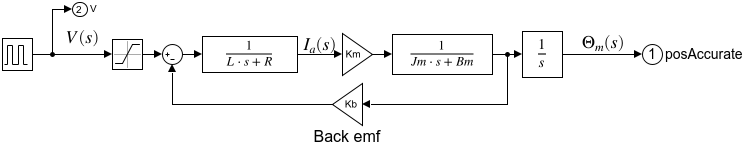
\includegraphics[width=\textwidth]{accurateManipulatorModel.slx.png}
    \caption{Accurate manipulator Simulink model}
    \label{fig:accurateManipulatorModel}
\end{figure}

\subsection{Simplified model (Task 2)}
\label{subsec:simplified-model}
After some manipulation of the \nameref{subsec:accurate-model} and neglecting
the electrical time constant $\frac{L}{R}<<\frac{J_m}{B_m}$ \cite{SingleLink}
one can obtain the simplified model of the single-link manipulator shown in
\autoref{fig:simplifiedManipulatorModel}.

\begin{figure}
    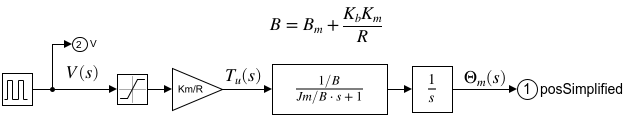
\includegraphics[width=\textwidth]{simplifiedManipulatorModel.slx.png}
    \caption{Simplified manipulator Simulink model}
    \label{fig:simplifiedManipulatorModel}
\end{figure}

\subsection{Comparison}
These two models have been compared by means of a simulation carried out in
Simulink. Which shows the system response to a pulse input.
\autoref{fig:modelAccurateVsSimplified} shows the results of this comparison.
It is easy to appreciate that the simplified model is sufficiently accurate to
be used as the single-link manipulator model. Its computational efficiency and
simplicity make it a better choice than the accurate model for the rest of the
report simulations.

\begin{figure}
    \centering
    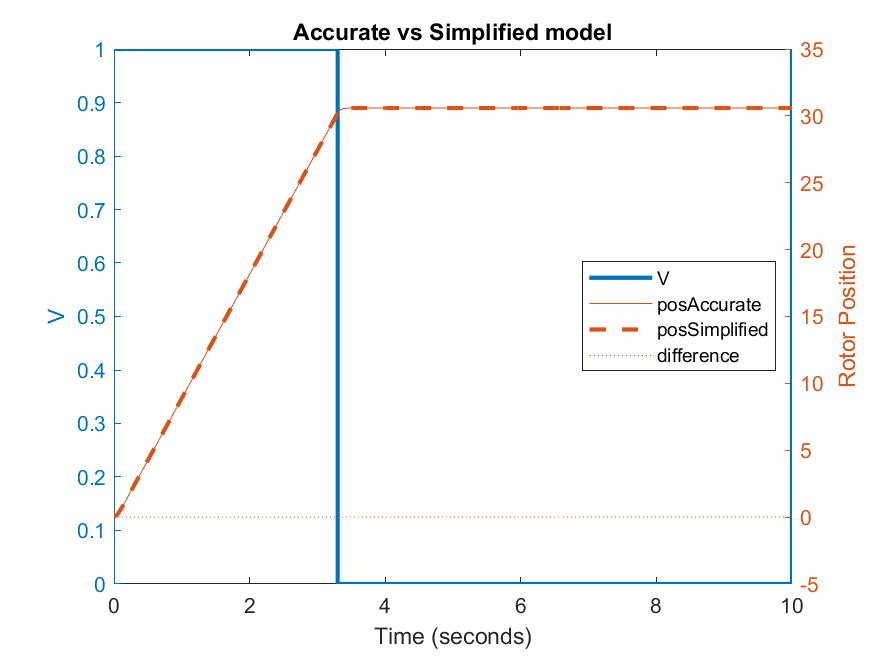
\includegraphics[width=.6\textwidth]{modelAccurateVsSimplified.png}
    \caption{Comparison of accurate and simplified single-link manipulator models}
    \label{fig:modelAccurateVsSimplified}
\end{figure}
\section{PD controller (Task 3)}
\label{sec:pd}

A PD controller has been designed so it satisfies the requirements shown in
\autoref{table:pd-requirements} for the cubic polynomial trajectory
\cite{TrajGener} described by \autoref{eqn:cubic-trajectory}. The controller
model is shown in \autoref{fig:PD}, the tuning of the control parameters is
described in \autoref{subsec:pd-tuning} and its behaviour in
\autoref{subsec:pd-behaviour}

\begin{equation}
    \text{Cubic polynomial trajectory } q(t) = 
    \begin{cases}
        1.5 t^2 - t^3 & t \leq 1 \\
        0.5 & \text{otherwise}
    \end{cases}
    \label{eqn:cubic-trajectory}
\end{equation}

\begin{table}
    \centering
    \begin{tabular}{c | c}
        Requirement & Value \\ \hline
        Maximal control error & $[0.01, 0.005]$
    \end{tabular}
    \\ [1ex]
    \caption{PD controller requirements}
    \label{table:pd-requirements}
\end{table}

\begin{figure}
    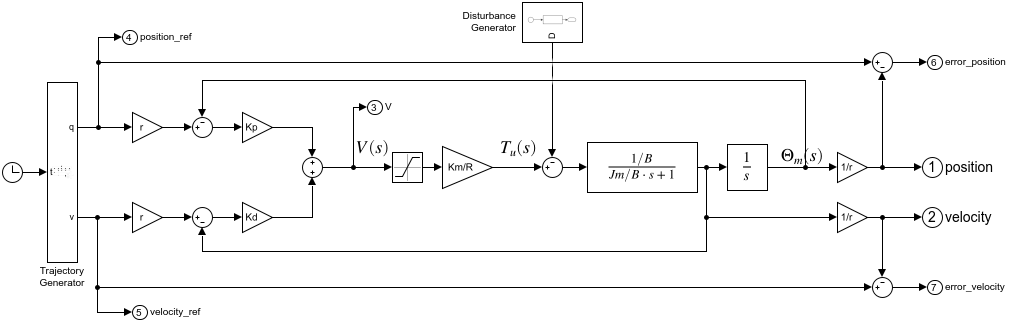
\includegraphics[width=\textwidth]{PD.slx.png}
    \caption{PD controller Simulink model}
    \label{fig:PD}
\end{figure}

\subsection{Tuning}
\label{subsec:pd-tuning}
In robotics the required dynamics should usually be possibly fast, but without
overshoots, this implies critical damping, i.e. $\zeta = 1$ \cite{SingleLink}.
That leaves the speed of response of the control system $\omega$ as the only
variable. Which is tuned in order to meet the requirements of
\autoref{table:pd-requirements}.

In order to do so, the model has been simulated with several values of $\omega$
and the maximum control error has been recorded. This maximum control error
corresponds to the maximum velocity reference, which in case of the cubic
trajectory corresponds to $t = t_f/2$ being $t$ the time and $t_f$ the end time
of the trajectory. This is exactly the middle of the movement.

\autoref{table:pd-tuning} shows the different values of the maximal control
error when modifying $\omega$. The value of $\omega = 45$ is therefore chosen to
be used for the rest of the section as it is the lowest value that satisfies
the requirements. The control system gains are calculated as described in
\citetitle{SingleLink} \cite{SingleLink} and summarized in \autoref{table:pd-constants}.

\begin{table}
    \centering
    \begin{tabular}{c | c}
        $\omega$ & Maximal control error \\ \hline\hline
        $50$ & $0.007357$ \\ \hline
        $45$ & $0.009069$ \\ \hline
        $40$ & $0.011474$ \\ \hline
    \end{tabular}
    \\ [1ex]
    \caption{PD controller tuning}
    \label{table:pd-tuning}
\end{table}

\begin{table}
    \centering
    \begin{tabular}{c | c}
        Variable & Value \\ \hline\hline
        $\omega$ & $45$ \\ \hline
        $K_p$ & $8.940857$ \\ \hline
        $K_d$ & $0.259476$ \\ \hline
    \end{tabular}
    \\ [1ex]
    \caption{PD controller parameters}
    \label{table:pd-constants}
\end{table}

\subsection{Behaviour}
\label{subsec:pd-behaviour}
The behaviour of the PD control system has been checked for the step change of
constant reference trajectory from $0$ to $0.5\text{ rad}$ as shown in
\autoref{fig:PD_step}. We obtain the expected critically damped response.

\begin{figure}
    \centering
    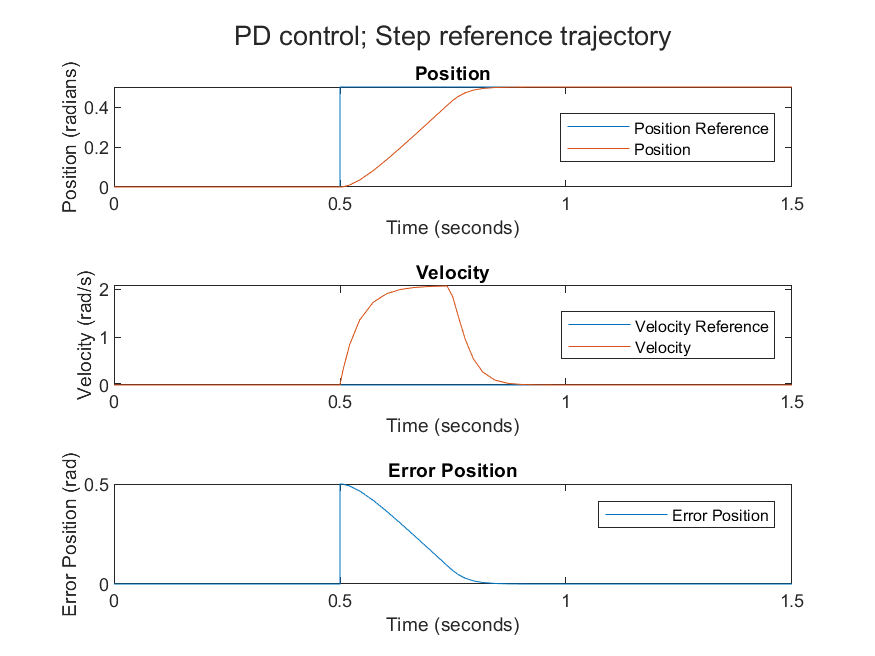
\includegraphics[width=.7\textwidth]{PD_step.png}
    \caption{Behaviour of the PD control system for the step change of constant reference trajectory from $0$ to $0.5\text{ rad}$}
    \label{fig:PD_step}
\end{figure}

\subsubsection{Undisturbed (Task 4)}
\label{subsubsec:pd-undisturbed}
The response of the PD control system has been also tested for the cubic
reference trajectory described by \autoref{eqn:cubic-trajectory} and the LSPB
\cite{TrajGener} reference trajectory described by
\autoref{eqn:LSPB-trajectory}. The results are shown in \autoref{fig:PD_cubic}
and \autoref{fig:PD_LSPB}, respectively.

Both trajectories show the expected curves for both, position and velocity. The
position error is directly related to the velocity reference and the
requirements specified in \autoref{table:pd-requirements}. It is worth to
mention that the position error for the LSPB trajectory is significantly
smaller (almost halve) than the one for the cubic polynomial trajectory. Being
both trajectory position curves quite similar this is an advantage for the LSPB
trajectory.

\begin{equation}
    \text{LSPB trajectory } q(t) = 
    \begin{cases}
        1.5625 t^2 & t \leq 0.2 \\
        0.0625 + 0.625 (t-0.2) & 0.2 \geq t \leq 0.8 \\
        0.5 - 1.5625 (t-0.6)^2 & 0.1 \geq t \leq 1 \\
        0.5 & \text{otherwise}
    \end{cases}
    \label{eqn:LSPB-trajectory}
\end{equation}

\begin{figure}
    \centering
    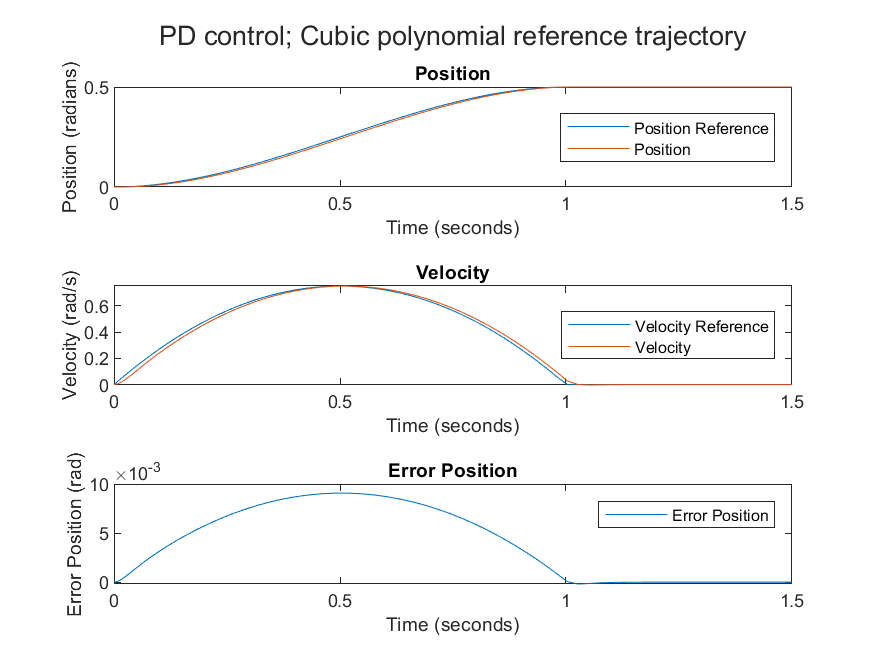
\includegraphics[width=.7\textwidth]{PD_cubic.png}
    \caption{PD control system response for the cubic polynomial trajectory}
    \label{fig:PD_cubic}
\end{figure}

\begin{figure}
    \centering
    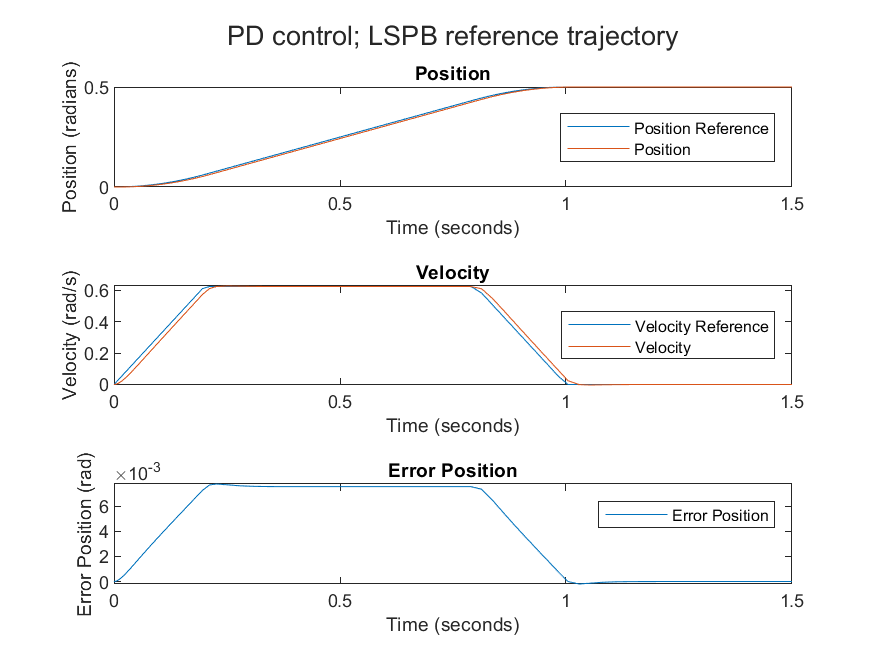
\includegraphics[width=.7\textwidth]{PD_LSPB.png}
    \caption{PD control system response for the LSPB trajectory}
    \label{fig:PD_LSPB}
\end{figure}

\subsubsection{Disturbed (Task 5)}
\label{subsubsec:pd-disturbed}
% \begin{minipage}{0.25\textwidth}
Finally, the response of the PD control system has been tested again in a
disturbed scenario with the two reference trajectories already mentioned. The
load disturbance tested is equal to $\tau_l/r = 2 N\cdot m$.
\autoref{fig:PD_cubic_disturbed} shows the results for the cubic polynomial
trajectory and \autoref{fig:PD_LSPB_disturbed} shows the results for the LSPB
trajectory.

Unlike in the undisturbed scenario, both simulations present a steady state
error in position. Being this error equal for both trajectories with a value of
$0.01379\text{ rad}$. Which matches with the equation for the steady state of a
PD control system derived in \citetitle{SingleLink} \cite{SingleLink}.
% \end{minipage}
% \begin{minipage}{0.7\textwidth}
\begin{figure}[h]
    \centering
    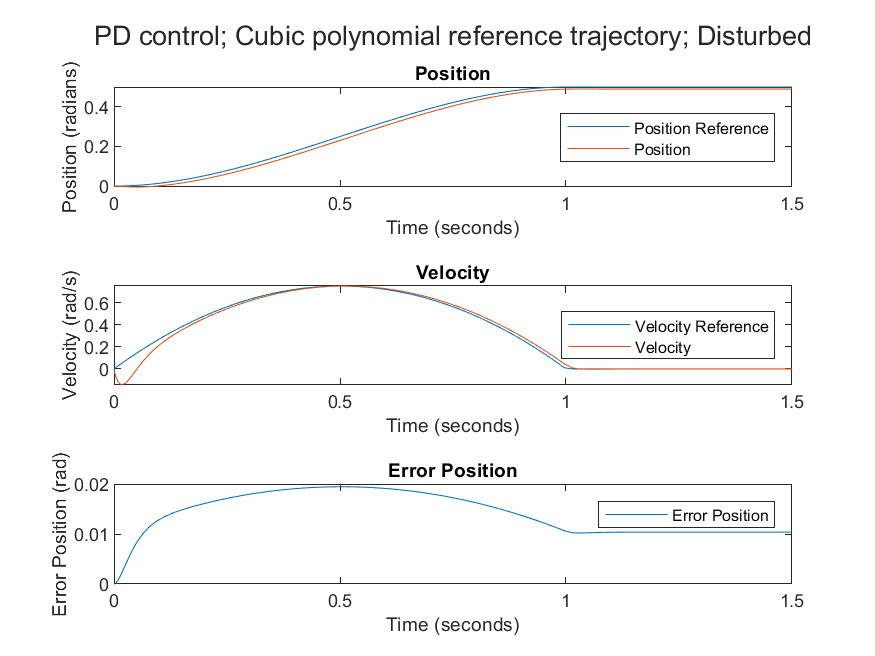
\includegraphics[width=.7\textwidth]{PD_cubic_disturbed.png}
    \caption{PD control system response for the cubic polynomial trajectory
    with disturbance}
    \label{fig:PD_cubic_disturbed}
\end{figure}
% \end{minipage}

\begin{figure}[h]
    \centering
    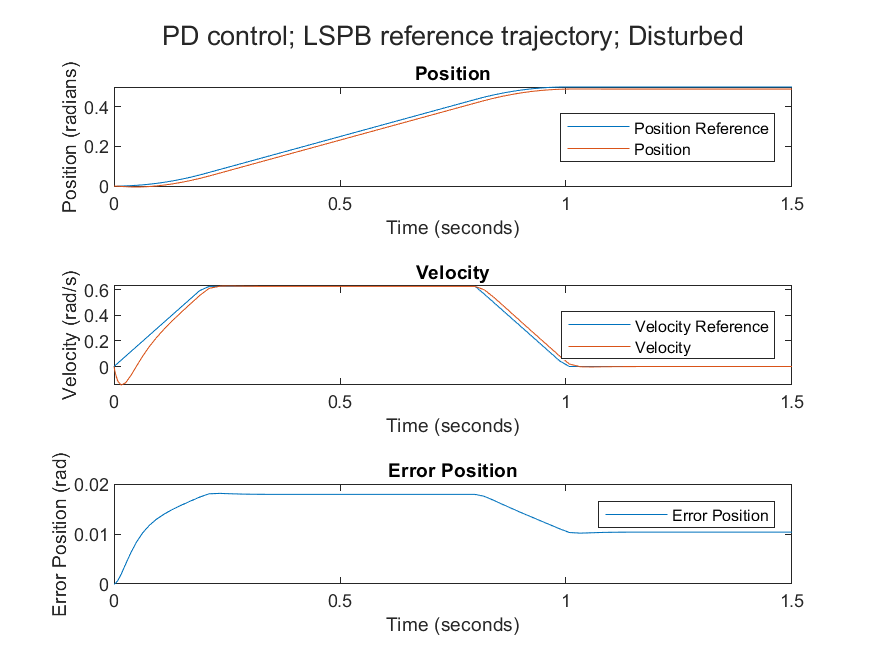
\includegraphics[width=.7\textwidth]{PD_LSPB_disturbed.png}
    \caption{PD control system response for the LSPB trajectory with disturbance}
    \label{fig:PD_LSPB_disturbed}
\end{figure}
\section{PID controller (Task 6)}
\label{sec:pd}

A PID controller has been designed so it satisfies the requirements shown in
\autoref{table:pd-requirements} for the cubic polynomial trajectory described
by \autoref{eqn:cubic-trajectory}. The \emph{back-calculation} anti-windup loop
has been implemented. The controller model is shown in \autoref{fig:PID}, the
tuning of the control parameters is described in \autoref{subsec:pid-tuning}
and its behaviour in \autoref{subsec:pid-behaviour}

\begin{figure}
    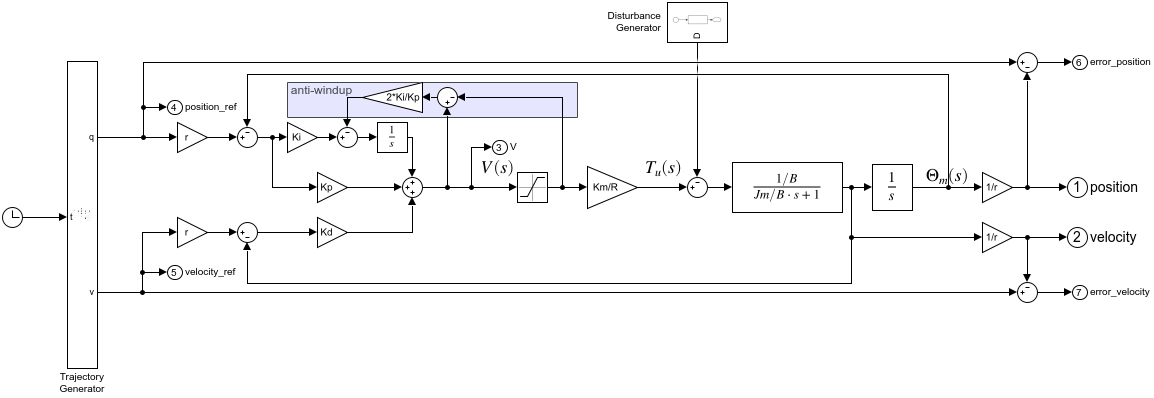
\includegraphics[width=\textwidth]{PID.slx.png}
    \caption{PID controller Simulink model}
    \label{fig:PID}
\end{figure}

\subsection{Tuning}
\label{subsec:pid-tuning}
As in \autoref{subsec:pd-tuning}, a critically damped system is desired and the
speed of the control system $\omega$ is tuned by iterative simulation.

\autoref{table:pid-tuning} shows the different values of the maximal control
error when modifying $\omega$. The value of $\omega = 18$ is therefore chosen to
be used for the rest of the section as it is the lowest value that satisfies
the requirements. The control system gains are calculated as described in
\citetitle{SingleLink} \cite{SingleLink} and the selected anti-windup gain is
$K=2*K_i/K_p$. A bit higher than the recommended as the critically dampening
behaviour is desired, avoiding in this way overshooting. All the gains are
summarized in \autoref{table:pid-constants}.

It is worth to mention that PID control has significantly lower $K_p$ and
$K_d$ gains for the same maximal error requirement.

\begin{table}
    \centering
    \begin{tabular}{c | c}
        $\omega$ & Maximal control error \\ \hline\hline
        $20$ & $0.007152$ \\ \hline
        $18$ & $0.009417$ \\ \hline
        $17$ & $0.011001$ \\ \hline
        $15$ & $0.015163$ \\ \hline
    \end{tabular}
    \\ [1ex]
    \caption{PID controller tuning}
    \label{table:pid-tuning}
\end{table}

\begin{table}
    \centering
    \begin{tabular}{c | c}
        Variable & Value \\ \hline\hline
        $\omega$ & $18$ \\ \hline
        $K_p$ & $4.291611$ \\ \hline
        $K_d$ & $0.130528$ \\ \hline
        $K_i$ & $25.749669$ \\ \hline
        $K_{anti-windup}$ & $12$ \\ \hline
    \end{tabular}
    \\ [1ex]
    \caption{PID controller parameters}
    \label{table:pid-constants}
\end{table}

\subsection{Behaviour}
\label{subsec:pid-behaviour}
The behaviour of the PID control system has been checked for the step change of
constant reference trajectory from $0$ to $0.5\text{ rad}$ as shown in
\autoref{fig:PID_step}. We obtain the expected damped response,
ensured by our selected anti-windup gain. During the simulations, it was proven
that a lower anti-windup gain resulted in an appreciable overshoot.

\begin{figure}
    \centering
    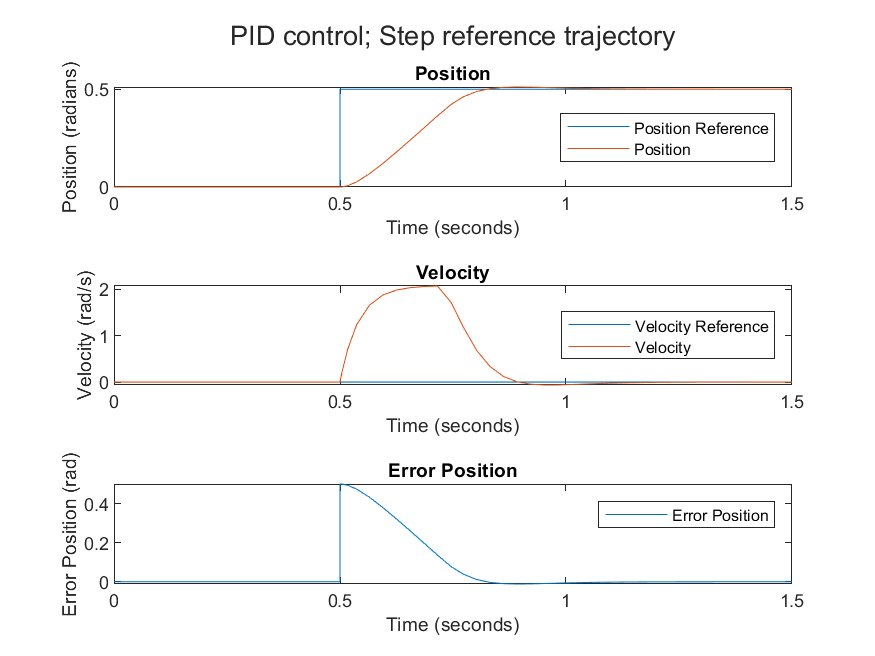
\includegraphics[width=.7\textwidth]{PID_step.png}
    \caption{Behaviour of the PID control system for the step change of constant reference trajectory from $0$ to $0.5\text{ rad}$}
    \label{fig:PID_step}
\end{figure}

\subsubsection{Undisturbed}
The response of the PID control system has been also tested for the cubic
reference trajectory described by \autoref{eqn:cubic-trajectory} and the LSPB
reference trajectory described by \autoref{eqn:LSPB-trajectory}. The results
are shown in \autoref{fig:PID_cubic} and \autoref{fig:PID_LSPB}, respectively.

Unlike in the analogous PD scenario described in
\autoref{subsubsec:pd-undisturbed}, LSPB trajectory shows a greater error than
cubic polynomial. Even with a lower anti-windup gain. Which proves that an
optimal trajectory will depend greatly on the control system.

\begin{figure}
    \centering
    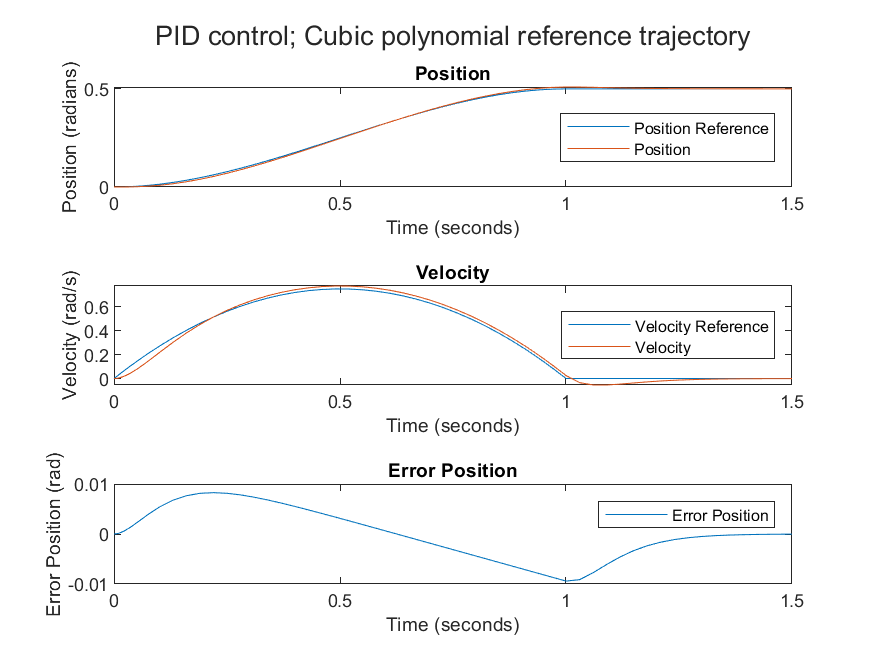
\includegraphics[width=.7\textwidth]{PID_cubic.png}
    \caption{PID control system response for the cubic polynomial trajectory. Error position is the difference between the position reference and the recorded arm position. Being positive when the reference position is greater than the recorded one, negative otherwise.}
    \label{fig:PID_cubic}
\end{figure}

\begin{figure}
    \centering
    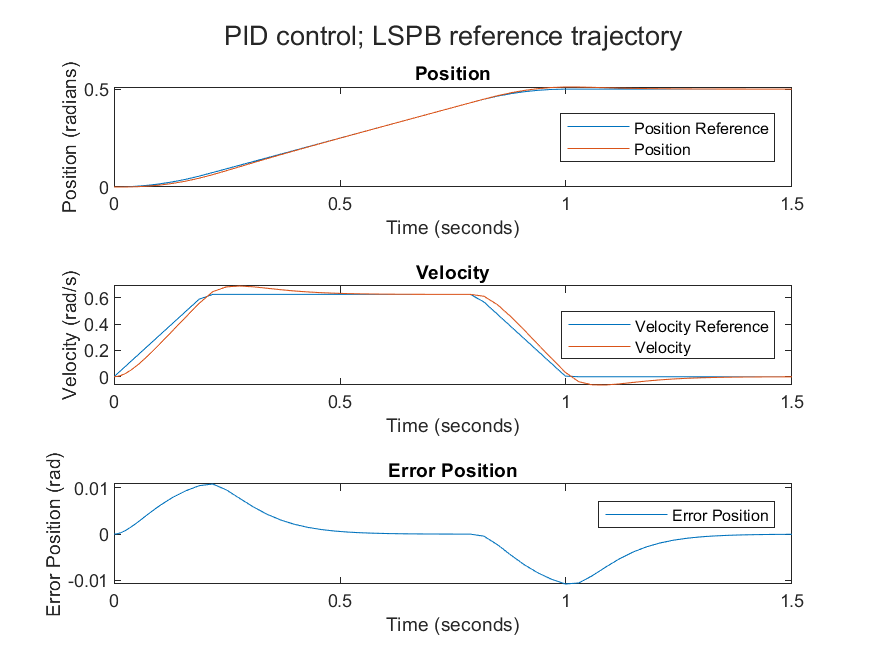
\includegraphics[width=.7\textwidth]{PID_LSPB.png}
    \caption{PID control system response for the LSPB trajectory. Error position is the difference between the position reference and the recorded arm position. Being positive when the reference position is greater than the recorded one, negative otherwise.}
    \label{fig:PID_LSPB}
\end{figure}

\subsubsection{Disturbed}
The response of the PID control system has been tested again in a disturbed
scenario with the two reference trajectories already mentioned. The load
disturbance tested is equal to $\tau_l/r = 2 N\cdot m$ as in
\autoref{subsubsec:pd-disturbed}. \autoref{fig:PID_cubic_disturbed} shows the
results for the cubic polynomial trajectory and
\autoref{fig:PID_LSPB_disturbed} shows the results for the LSPB trajectory.

Unlike again in the analogous PD scenario described in
\autoref{subsubsec:pd-undisturbed}, the steady state error is effectively $0$
with PID control.

\begin{figure}[h]
    \centering
    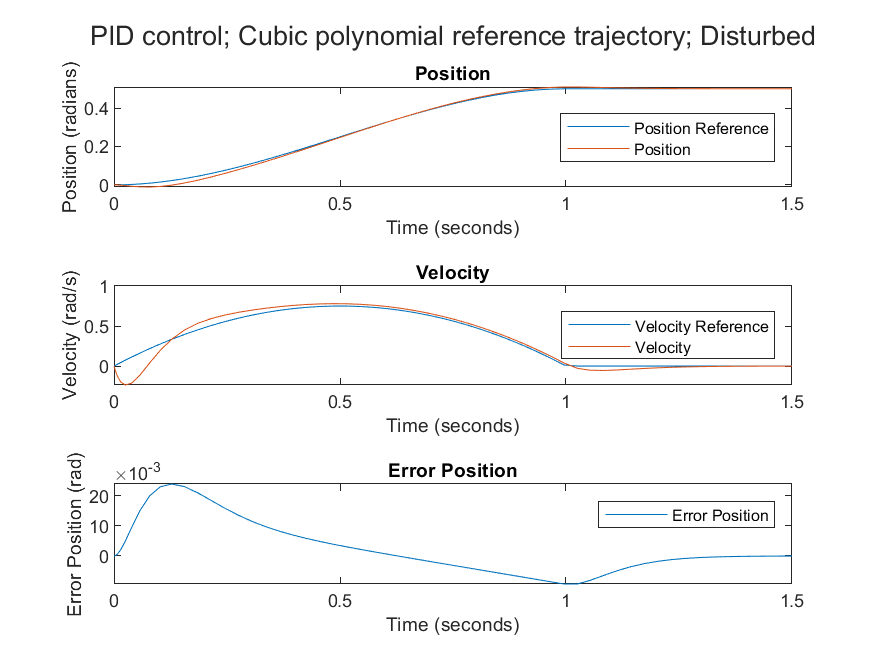
\includegraphics[width=.7\textwidth]{PID_cubic_disturbed.png}
    \caption{PID control system response for the cubic polynomial trajectory
    with disturbance. Error position is the difference between the position reference and the recorded arm position. Being positive when the reference position is greater than the recorded one, negative otherwise.}
    \label{fig:PID_cubic_disturbed}
\end{figure}

\begin{figure}[h]
    \centering
    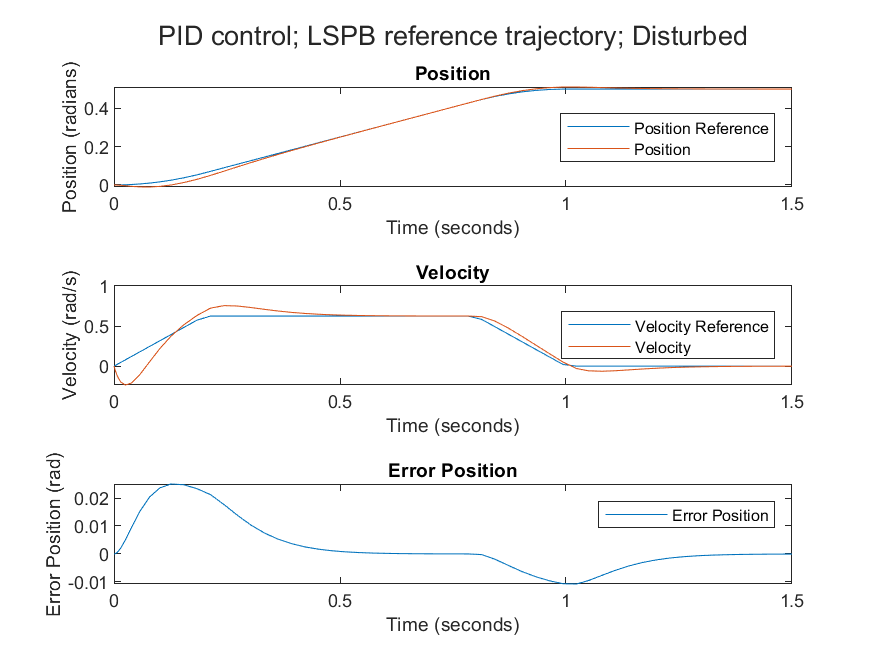
\includegraphics[width=.7\textwidth]{PID_LSPB_disturbed.png}
    \caption{PID control system response for the LSPB trajectory with disturbance. Error position is the difference between the position reference and the recorded arm position. Being positive when the reference position is greater than the recorded one, negative otherwise.}
    \label{fig:PID_LSPB_disturbed}
\end{figure}

\clearpage
\subsection{Feedforward (Task 7)}
Finally, the effect of the feedforward action has been tested for the
sinusoidal reference trajectory described in
\autoref{eqn:sinusoidal-trajectory}. 

\begin{equation}
    \text{Sinusoidal trajectory } q(t) = 0.25*\sin\left(\pi*6.8\right)
    \label{eqn:sinusoidal-trajectory}
\end{equation}

\autoref{fig:PIDfeedforward} illustrates the model of the PID control system
with feedforward action that was used for the simulations.
\autoref{fig:PIDfeedforward_sinusoidal} shows the comparison of using
feedforward action against not using it.

One can realize at first sight that the control system with feedforward action
has a lower error than the one without it. With a closer look one can also see
that both with and without feedforward action steady state trajectories have
the same sinusoidal amplitude and frequency. But the phase of the control
system with feedforward action is better aligned with the reference trajectory.
Which is the cause for the lower error.

Additionally, the control system with feedforward action did not
suffer the same transient state that can be observed in the control system
without feedforward, where the error is even higher. This means that the
feedforward effect will be even more important with random oscillations like
noise in the reference trajectory.

\begin{figure}
    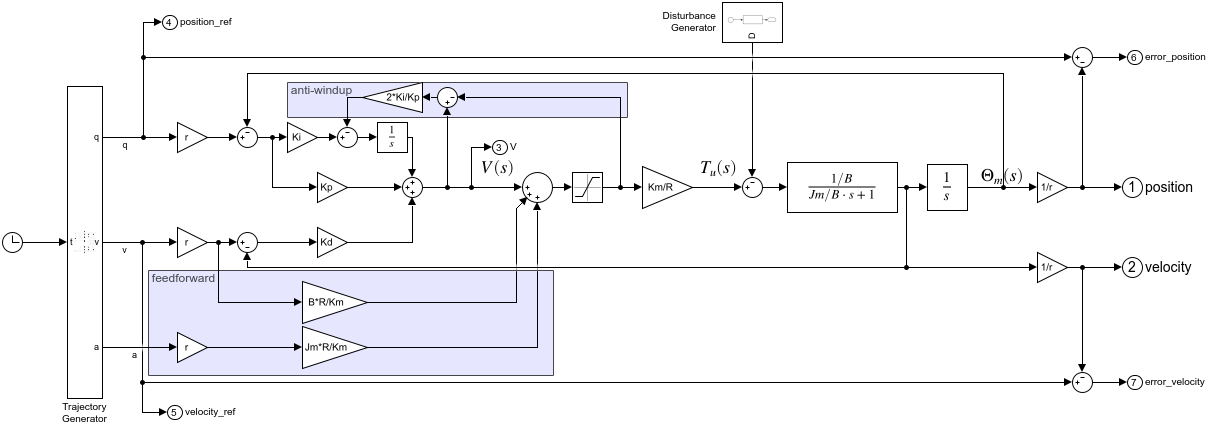
\includegraphics[width=\textwidth]{PIDfeedforward.slx.png}
    \caption{PID controller with feedforward Simulink model}
    \label{fig:PIDfeedforward}
\end{figure}

\begin{figure}[h]
    \centering
    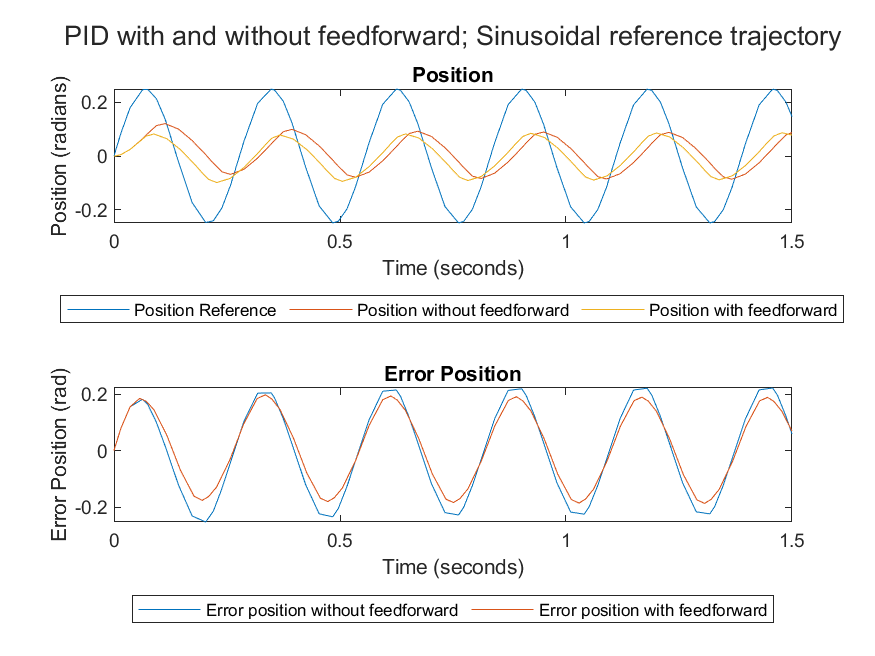
\includegraphics[width=.7\textwidth]{PIDfeedforward_sinusoidal.png}
    \caption{PID control response with and without feedforward action for a sinusoidal trajectory. Error position is the difference between the position reference and the recorded arm position. Being positive when the reference position is greater than the recorded one, negative otherwise.}
    \label{fig:PIDfeedforward_sinusoidal}
\end{figure}
\section{Conclusions}

Several control system models have been developed and simulated during the
realization of this homework. Key learnings that have been extracted: Optimal
trajectory is very sensible to the control system used; Feedforward action
aligns the trajectory of the manipulator with the oscillations of the reference
trajectory.


  % ***************************************************************************
  %                              Appendices
  % ***************************************************************************
  \IfFileExists{./appendices.tex}{
    \appendix
    \input{appendices}
    \unappendix
    \clearpage
  }

  % ***************************************************************************
  %                              Bibliography
  % ***************************************************************************
  \singlespace
  \printbibliography[%
    % heading=bibintoc,%
    title={References}%
  ]

\end{document}